The GMCF performance evaluation discussed in Section~\ref{sec:GMCFLESEval} was
the first ever to be conducted on the framework. The results discussed in the
evaluation were the final best results obtained after a number of changes were
made to the framework to improve performance.

Also, during development of the GMCF parallelised LES, an unusual bug was
encountered caused by Fortran and C++ interoperability through POSIX threads.
The bug is not framework specific but will be discussed in
Section~\ref{sec:fortrancppinteroperability} as it is applicable to any
application using POSIX threads to call Fortran subroutines.

\subsection{Performance improvements}

\begin{figure}
    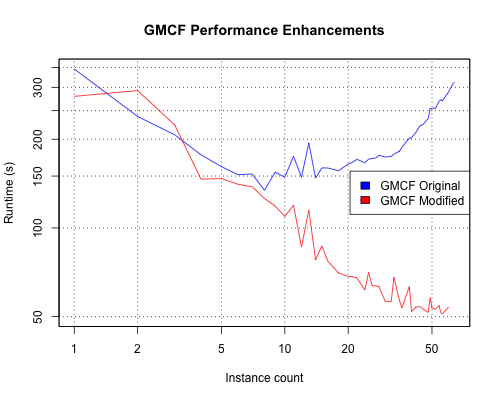
\includegraphics[width=0.5\textwidth]
    {graphs/GMCF-before-after-fixed-area.png}
    \caption{GMCF Before and After}
    \label{fig:gmcfbeforeandafter}
\end{figure}

Figure~\ref{fig:gmcfbeforeandafter} shows the original GMCF performance results
alongside the best results for a fixed area run. As is clear from the graph,
GMCF was suffering from scalability issues, with the runtime increasing above
ten threads and causing a bathtub curve.

\subsubsection{Global Reduction}

\subsubsection{Spin locks and busy waiting}

\subsubsection{Thread Pinning}

\subsubsection{Miscellaneous Changes}

\subsection{Fortran and C++ interoperability issue}
\label{sec:fortrancppinteroperability}

That weird Fortran/C++ stack array above a certain size sharing thing.
